\documentclass{article}
% Gives us lovely headers
\usepackage{fancyhdr}
% Means you don't have to put \\ to start a new line.
\usepackage[parfill]{parskip}

% For diagrams
\usepackage{tikz}
\usetikzlibrary{shapes, patterns}
\definecolor{light-gray}{gray}{0.95}

\begin{document}
% Meta
\author{Chris Williamson, Todd Davies}
\title{COMP15111 Notes}
\rhead{COMP15111 Notes}

\maketitle
\tableofcontents
\newpage

\section{Lecture 1: Introduction}
\subsection{A Computational Model}
The simplest, earliest, commonest, most important computational model is the \textbf{Von-Neumann Imperative Procedural Computer Model}

According to this model, a computer can:
\begin{enumerate}
	\item Store information
	\item Manipulate the stored information
	\item Make decisions depending on the stored information
\end{enumerate}

\subsection{Simple View Of A Computer}
\[
	Memory \Leftrightarrow Bus \Leftrightarrow Processor
\]

\subsubsection{Memory}
Memory is a set of locations which can hold information, such as numbers(or programs). Each memory location has a unique (numerical) address, and there are typically thousands of millions of different locations. There are various ways of depicting memory; a common one is a 'hex dump' that often looks something like this: \marginpar{\raggedright Run the command {\it hexdump} to generate hexdumps.}

\begin{tabular}{l l l}
	Address     &	Values (8 bit numbers)	&	Characters\\
	00000000	&	48 65 6c 6c 6f 0a		&	Hello.\\
\end{tabular}

Each item that is in the memory has a unique address.

\subsubsection{Bus}
A bus is a bidirectional communication path. It is able to transmit addresses and numbers between components inside the computer.

\subsubsection{Processor}
The processor obeys a sequence of instructions, commonly referred to as a program.
Historically the processor was often referred to as a CPU, however, this is inappropriate nowadays since typical processors consist of several processing cores.

\subsection{Three-address instructions}
Every kind of processor has a different set of instructions, real world examples include: Pentium, ARM and others

Each three-address instruction:
\begin{enumerate}
	\item Copies the values from any two memory locations and sends them to the processor (source operands)
	\item Copies some operation e.g. adds the copied numbers together
	\item Copies the result back from the processor into a third memory location (destination operand)
\end{enumerate}

For example, if we wanted to convert the Java code $sum = a + b;$ into a three-address instruction we would:
\begin{enumerate}
	\item Identify the two {\it source operands}: $a$ holds 2, $b$ holds 3
	\item Perform the {\it operation}: 2 + 3 = 5
	\item Let the variable $sum$ equal the answer 5. This is the {\it destination operand}
\end{enumerate}

\subsubsection{Three address example}
{\bf Question:} Convert the Java code {\it product = c * d;} into the three-address style and draw a two box view of it.

First we need to re-write the Java code in the three-address style:
\[
	product \leftarrow c * d
\]
Now we can draw the box view of it:
\begin{center}
    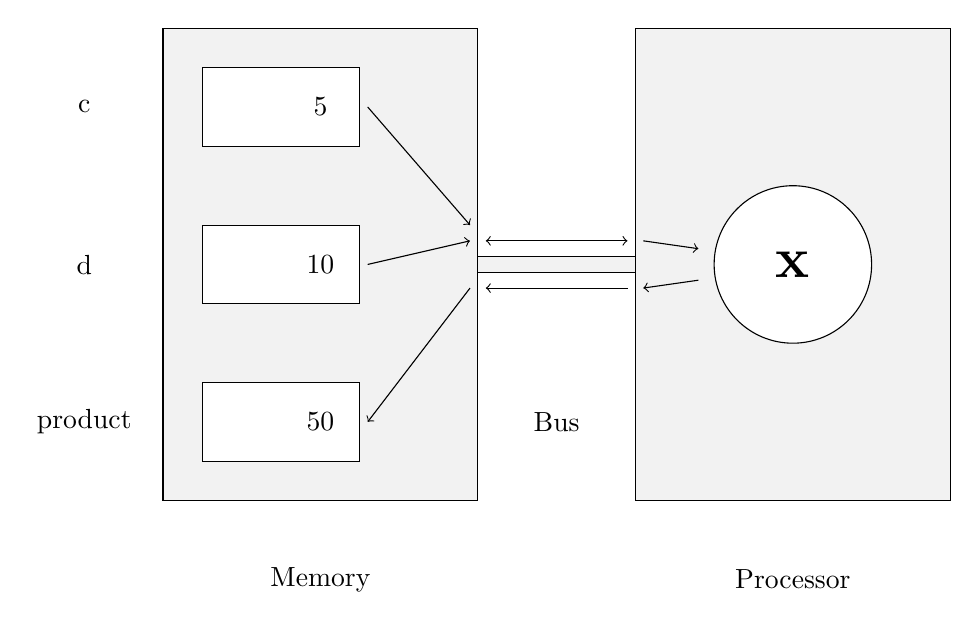
\begin{tikzpicture}
    	% Memory box
    	\draw [fill=light-gray] (-5,  3) rectangle (-1, -3);
    	% Memory label
    	\node at (-3, -4) {Memory};
    	% 5 box
    	\draw [fill=white] (-4.5,  2.5) rectangle (-2.5, 1.5);
    	\node at (-3, 2) {5};
    	% 5 to bus arrow
    	\draw [->] (-2.4, 2) -- (-1.1, 0.5);
    	% c label
    	\node at (-6, 2) {c};
    	% 10 box
    	\draw [fill=white] (-4.5,  0.5) rectangle (-2.5, -0.5);
    	\node at (-3, 0) {10};
    	% 10 to bus arrow
    	\draw [->] (-2.4, 0) -- (-1.1, 0.3);
    	% d label
    	\node at (-6, 0) {d};
    	% 50 box
    	\draw [fill=white] (-4.5,  -1.5) rectangle (-2.5, -2.5);
    	\node at (-3, -2) {50};
    	% Bus to 50 arrow
    	\draw [->] (-1.1, -0.3) -- (-2.4, -2);
    	% product label
    	\node at (-6, -2) {product};
    	% Bus rectangle
    	\draw [fill=light-gray] (-1, 0.1) rectangle (1, -0.1);
    	% Bottom bus arrow
    	\draw [<-] (-0.9, -0.3) -- (0.9, -0.3);
    	% Top bus arrow
    	\draw [<->] (-0.9, 0.3) -- (0.9, 0.3);
    	% Bus label
    	\node at (0, -2) {Bus};
    	% Processor box
		\draw [fill=light-gray] (1,  3) rectangle (5, -3);
		% Bus to processor
    	\draw [->] (1.1, 0.3) -- (1.8, 0.2);
    	% Processor to bus
    	\draw [<-] (1.1, -0.3) -- (1.8, -0.2);
		% Processor label
    	\node at (3, -4) {Processor};
    	% Multiplication circle
    	\draw [fill=white] (3, 0) circle [radius=1];
    	\node at (3, 0) {\huge \bf x};
    \end{tikzpicture}
\end{center}
% TODO: Discuss the memory bottleneck mentioned in Javier's notes.

\subsection{Registers}
Reduce accesses to main memory by using registers:
\begin{enumerate}
\item Very small, very fast memory within the processor
\item Each register can hold a single value
\end{enumerate}
Processors contain up to a few dozen registers e.g. ARM: 16 registers - R0 to R15

\subsection{Instruction Styles}
Make instructions as simple as possible while allowing for the best use of registers. One-address style (e.g. Intel Pentium):
\begin{enumerate}
	\item Only use (at most) 1 memory location in each instruction
	\item Use registers for the other operands
\end{enumerate}

\[
	register \leftarrow register + memory location
\]

\textbf{Load-store} style (e.g. ARM): Use registers for all three operands

\[
	register \leftarrow register + register
\]

So we need extra instructions to get at memory locations:
\begin{enumerate}
	\item \textbf{Load} (from memory): register \(\leftarrow\) memory location
	\item \textbf{Store} (to memory): memory location \(\rightarrow\) register
\end{enumerate}

Sum = a + b + c;
% TODO: Clean this into a table or something
Becomes:
Register1 \(\leftarrow\) a                      (i.e. load from a)\\
Register2 \(\leftarrow\) b                      (i.e. load from b)\\
Register3 \(\leftarrow\) register 1 + register2 (i.e. a+b)\\
Register4 \(\leftarrow\) c                      (i.e. load from c)\\
Register5 \(\leftarrow\) register3 + register4  (i.e. (a+b)+c)\\
sum \(\rightarrow\) register5                   (i.e. store to sum)\\
One load or store instruction per variable (a, b, c, sum)\\
One arithmetic instruction per operation (+, +)\\
Lots of very simple, very fast instructions

\section{Lecture 2}
Computers obey programs which are sequences of instructions. Instructions are coded as values in memory. The sequences are held in memory adjacent memory locations. Values in memory can be interpreted as:
\begin{itemize}
	\item Numbers (in several different ways)
	\item Instructions
	\item Text
	\item Colours
	\item Music
	\item Anything you want
\end{itemize}
Values are often represented as numbers for convenience.

\subsection{Assembly Language}
Assembly language is a means of representing machine instructions in a human readable form.\\
Each type of processor has its own assembly language but they typically have a lot in common:
\begin{itemize}
	\item A mnemonic – specifies the type of operation
	\item A destination – a register on this case
	\item And one or more sources – also registers
	\item Possibly with a comment too
\end{itemize}

\subsection{ARM instructions}
ARM has many instructions but we only need three categories:
\begin{itemize}
	\item Memory operations
	\item Processing operations
	\item Control flow
\end{itemize}
Memory operation move data between the memory and the registers. Processing operations perform calculations using value already in registers. Control flow instructions are used to make decisions, repeat operations etc.

\subsection{ARM memory instructions}
Memory operations load a register from the memory or store a register value to the memory.
% TODO: Clean this into a math/code/tabular environment or something.
e.g. LDR R1, a – means: R1 \(\leftarrow\) a\\
e.g. STR R5, sum – means: R5 \(\rightarrow\) sum (i.e. sum \(\leftarrow\) R5)\\

$a$ and $sum$ are aliases for the addresses of memory locations.

\subsection{ARM processing instructions}
Processing operations such as addition, subtraction, multiplication.

e.g. ADD R3, R1, R2 – means: R3 \(\leftarrow\) R1 + R2

\subsection{ARM control instructions}
Fundamentally, these are branches to other code sequences. Often, branches are made conditional to allow decisions to be made.

% TODO: Clean this into a math/code/tabular environment or something.
e.g. B somewhere – means: branch to ‘somewhere’\\
e.g. BEQ elsewhere – means: branch to ‘elsewhere’ IF ‘previous result’ was ‘equals’\\
e.g. BNE wherever – means: branch to ‘wherever’ IF ‘previous result’ was ‘not equal’\\

\subsection{Stored programs and the Program Counter}
A computer can make decisions, and choose which instructions to obey next depending upon the results of those decisions. How? First we need to see how the sequence of instructions is controlled. Von-Neumann Model: memory holds both instructions and numbers - \textbf{stored program} \textbf{Program Counter} (PC) register: holds the address of the memory location containing the next instruction to b obeyed (executed).

ARM uses register 15 as its PC

\subsection{Fetch-Execute Cycle}
Start with PC containing the address of (the memory location holding) the first instruction of a program.

Repeatedly:
\begin{enumerate}
	\item \textbf{Fetch}: copy the instruction, pointed to by the PC, from memory and set PC to point to the next instruction
	\item \textbf{Execute}:  obey the instruction (exactly as before)
\end{enumerate}
ARM:
\begin{enumerate}
	\item 'Resets' to (starts at) address 00000000
	\item Instructions each occupy 4 memory locations, so PC increases by 4 in each fetch
\end{enumerate}

\subsection{Decision Making}
Linear sequences of instructions are limiting. To make a decision, the computer must change (or not) to a
different sequence of instructions.

e.g. a 1 pound discount on items worth 20 pounds or more.
Decision: compare the total and 20 pounds to see if it is larger, then depending on result, either perform action or not.
Action: subtract 1 pound from the total.\\

Computers have no intelligence, so spell out details.
\textbf{Formalise}: if total \(\geq\) 20 pounds then subtract 1 pound from total\\
\textbf{Rewrite}: if total \(\textless\) 20 pounds then don’t\\
\textbf{subtract} 1 pound from total\\
Encode: as ARM instructions

\subsection{Compare And Branch}

\end{document}

